\chapter{重症患者的镇痛镇静}

\section{前沿学术综述}

重症医学科的重症患者往往因病重而难以自理,甚至口不能言,手不能动,但其仍然保留着对外界的感觉、记忆与意识。在昼夜灯光长明的病房里,自身伤病的疼痛,各种有创的检查治疗,全身满布的各种插管,陌生的环境,冰冷的机器设备,此起彼伏的报警声音,抢救时紧张的呼喊,频繁被惊扰的睡眠,相邻患者病情的突然恶化乃至死亡,对自己病情的忧虑以及对家人的思念与担心\ldots{}\ldots{}这一切都使得患者处于极度的“无助”和不断加深的“恐惧”感觉之中,可能构成对患者的恶性刺激,增加患者的痛苦,甚至使患者因为这种“无助与恐惧”而挣扎,危及生命安全。国外有学者调查表明,离开重症医学科的患者中,约有50%的患者对于其在重症医学科中的经历保留有痛苦的记忆,而70%以上的患者在重症医学科期间存在着焦虑与激惹
\protect\hyperlink{text00027.htmlux5cux23ch1-26}{\textsuperscript{{[}1{]}}}
。因此,重症医学工作者应该时刻牢记,我们在抢救生命、治疗疾病的过程中,必须同时注意尽可能减轻患者的痛苦与恐惧感,使患者不感知或者遗忘其在危重阶段的多种痛苦,以避免加重患者的病情或影响其接受治疗。

镇痛与镇静治疗是保护重症患者安全的重要手段。重症患者的疼痛与焦虑不但表现为感情与精神方面的无助与恐惧以及躯体疾病和手术伤口的疼痛和不适,更有诸多所谓“隐匿性疼痛”的袭扰:长时间卧床,各种各样的插管、引流管,医护人员反复的检查治疗,包括压眶反射、疼痛感觉检查及病变部位触诊、频繁的吸痰、机械通气时的“人机对抗”,等等,都会引起患者的焦虑与躁动,甚至会因此意外拔除气管插管、深静脉插管而危及生命。所以,重症医学科积极的镇痛与镇静治疗,不仅应该针对临床明显的疼痛与焦虑,还需要及时发现并处理各种“隐匿性”的疼痛与焦虑,防患于未然。

镇痛与镇静治疗还是抢救极度重症患者的必备步骤。自然界的许多生物在外部环境极端恶劣的情况下,往往被迫采取“冬眠”或“夏眠”的方式,将自身的代谢速率降至最低,等待外部环境的改善以恢复正常生机。在处理临床重症患者的过程中,有时我们面对非常顽固的低灌注、低氧合状态,一时很难迅速纠正,也不得不通过强力的镇痛、镇静等措施将患者的代谢消耗降至最低,待其他病理生理因素得到纠正之后,再逐渐降低镇痛、镇静强度,直至停止治疗。

国际上,重症医学建立发展之初,镇痛与镇静就是治疗的重要手段。当时,由于医疗知识的局限和诸如呼吸机等医疗设备的落后,在重症患者进入重症医学科后要常规给予镇静甚至肌松治疗,以增加患者对于各种治疗的耐受。但随着时间的推移、科技的进步和重症医学科学的发展,20世纪80年代之后,国外学者逐渐认识到过度镇静的种种弊端:自我保护反射削弱,机械通气时间延长,肺部感染增加,深静脉血栓形成,皮肤压疮,以及神经肌肉传导障碍等等,于是加强了对镇痛镇静治疗的研究,更加注重“适度”,讲求平衡,既往那种过度镇痛镇静的现象得到大幅度纠正。而恰在此时,我国的重症医学事业开始起步,受到当时国外“矫枉过正”的影响,我国的多数重症医学工作者对于重症医学科中患者的镇痛镇静治疗重视不够,甚至出现了危及患者生命的惨痛教训。20世纪90年代以后,国外的一些重症医学学会相继推出并不断更新了一系列镇痛镇静治疗指南
\protect\hyperlink{text00027.htmlux5cux23ch2-26}{\textsuperscript{{[}2{]}}}
,中华医学会重症医学分会也于2006年上半年推出了重症医学科重症患者镇痛与镇静治疗指南
\protect\hyperlink{text00027.htmlux5cux23ch3-26}{\textsuperscript{{[}3{]}}}
,其目的在于推广适度镇痛镇静的理念与方法,提高重症医学科中重症患者的整体治疗水平。

\section{临床问题}

\subsection{镇痛、镇静的目的和临床意义}

\subsubsection{疼痛、焦虑与躁动对重症患者有哪些危害?}

疼痛是因损伤或炎症刺激,或因情感痛苦而产生的一种不适的感觉,焦虑是一种强烈的忧虑,不确定或恐惧状态;躁动则是一种伴有不停动作的易激惹状态,或者说是一种伴随着挣扎动作的极度焦虑状态。

重症患者疼痛的诱发因素包括原发疾病、各种监测、治疗手段(显性因素)和长时间卧床制动、气管插管(隐匿因素)等。疼痛导致机体应激、睡眠不足和代谢改变,进而出现疲劳和定向力障碍,导致心动过速、组织耗氧增加、凝血过程异常、免疫抑制和分解代谢增加等。疼痛还可刺激疼痛区周围肌肉的保护性反应,导致全身肌肉僵直或痉挛等限制胸壁和膈肌运动,进而造成呼吸功能障碍。

50%以上的重症患者可能出现焦虑症状,其特征包括躯体症状(如心慌、出汗)和紧张感。

引起焦虑的原因均可以导致躁动。另外,某些药物的副作用、休克、低氧血症、低血糖、酒精及其他药物的戒断反应、机械通气不同步等,也是引起躁动的常见原因。研究显示,最易使重症患者焦虑、躁动的原因依次为:疼痛、失眠、经鼻或经口腔的各种插管、失去支配自身能力的恐惧感以及身体其他部位的各种管道限制活动。

躁动可导致患者与呼吸机对抗,使耗氧量增加,引起意外拔除身上各种装置和导管,甚至危及生命,所以应该及时发现躁动,积极寻找诱因,在实施镇静药物治疗之前积极纠正患者紊乱的生理状况,包括低氧血症、低血糖、低血压和疼痛等,并为患者营造舒适的人性化的环境,向患者解释病情及所实施治疗的目的和意义,尽可能使患者了解自己病情、参与治疗并积极配合。

\subsubsection{何谓镇痛与镇静治疗?}

镇痛治疗是指通过药物或(和)非药物手段(音乐、心理暗示、针刺等异位刺激,以及理疗等)以提升患者的痛觉阈值,减轻或消除患者的疼痛感觉。

镇静治疗是指借助于药物等手段使焦虑或(和)躁动的患者处于一种平静安详的状态。镇静治疗需要首先祛除一切可能导致焦虑/躁动的诱发因素,药物治疗应在此基础上进行。作为重症医学科中主要的镇静治疗手段,镇静药物治疗应能够使患者解除焦虑,安静而不再关注身边的痛苦恐惧,并且能够遗忘诸多恶性的刺激。

由于重症医学科中的许多患者都伴有躯体疾病的疼痛,因此在实施镇静治疗之前,应该有效地缓解患者的疼痛,镇痛是镇静治疗的基础。

\subsubsection{重症患者接受镇痛镇静治疗有何临床意义?}

镇痛与镇静治疗并不等同,镇痛是基础,镇静必须是在已祛除疼痛因素的基础之上帮助患者克服焦虑,是增加睡眠和遗忘的进一步治疗。

在镇痛镇静治疗之前,应尽量明确患者产生疼痛及焦虑激惹等症状的原因,尽可能采用各种非药物手段祛除或减轻一切可能的影响因素。镇痛与镇静治疗是特指应用药物手段以消除患者疼痛,减轻患者焦虑和激惹,催眠并诱导遗忘的治疗,其目的和意义在于:

(1)消除或减轻患者的疼痛及躯体不适感,减少不良刺激及交感神经系统的过度兴奋。

(2)帮助和改善患者睡眠,诱导遗忘,减少或消除患者对其在重症医学科治疗期间的痛苦记忆。

(3)减轻或消除患者的焦虑、激惹甚至谵妄,防止患者的无意识行为(如挣扎)干扰治疗,保护患者的生命安全。

(4)降低患者的代谢速率,减少其氧耗、氧需,使得受到损害的氧输送尽量能够满足机体组织氧耗的需求,并减轻各器官的代谢负担。

(5)对病情非常危重的患者,诱导并维持一种低代谢的“休眠”状态,尽可能地减少各种炎性介质的产生和释放,有助于减轻细胞与器官损伤。

\subsubsection{重症医学科镇静与麻醉镇静有什么异同?}

接受全身麻醉的患者多数为择期手术者,即使是急诊患者,一般也要求主要的生命体征趋于稳定。由于手术时间罕有超过24小时者,且手术操作的需要往往必须配合应用肌松药物,并使患者丧失一切感觉与意识,因此患者在短时间内所达到的镇痛镇静深度要大大超过重症患者,此时患者丧失了一切自我保护反射,丧失感觉运动及意识。而重症患者则不然,一方面其需要镇痛镇静的时间远远长于手术麻醉时间,另一方面其深度要求又必须尽可能保留其基本的生理防御反射和感觉运动功能;同时由于多器官功能障碍而往往需要合并多种治疗手段和药物,必须考虑彼此间的相互作用影响。因此重症患者具有镇痛镇静药物的累积剂量大,药代和药效动力学不稳定的特点,需要经常判断镇痛镇静程度并随时调整药物种类与剂量(表\ref{tab21-1})。

\begin{table}[htbp]
\centering
\caption{手术麻醉与重症医学科镇静的区别}
\label{tab21-1}
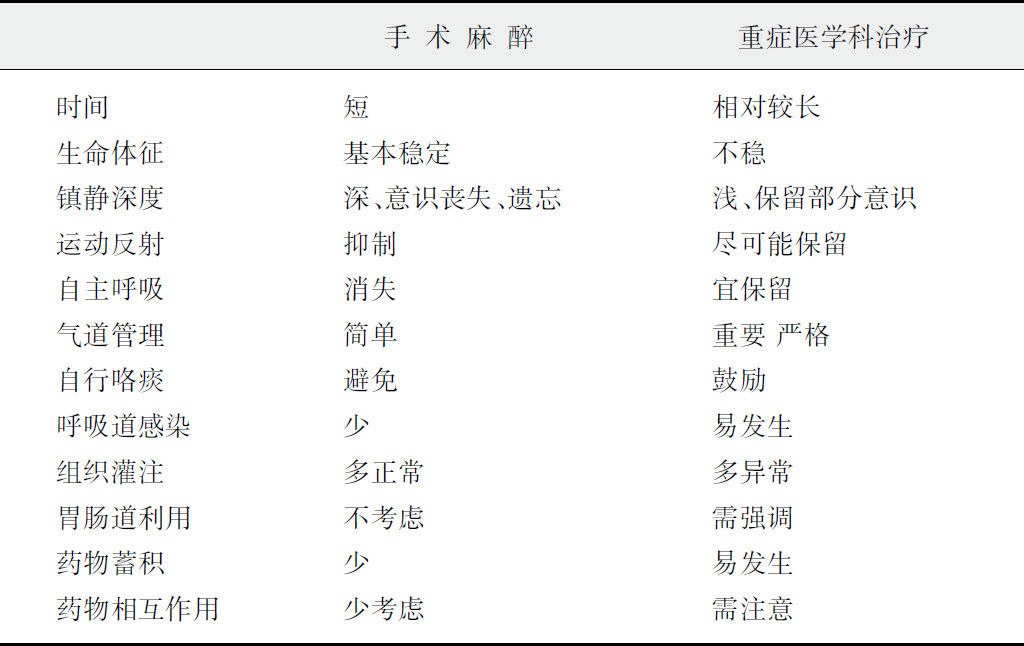
\includegraphics{./images/Image00226.jpg}
\end{table}

\subsection{镇痛镇静的临床评估}

\subsubsection{为什么要对重症患者进行疼痛和镇静状态评估?}

相对于全身麻醉,重症患者的镇痛镇静治疗更加强调“适度”的概念,因为“过度”与“不足”都可能给患者带来损害。为此,需要对重症患者疼痛与意识状态及镇痛镇静疗效进行准确的评价。

就目前我国的大部分重症医学科而言,镇痛不足是普遍现象,其危害已如前述,但镇静过度也同样对患者不利:难以观察患者的意识状态及检查感觉运动和反射;神经肌肉的废用导致神经肌肉突触传导障碍,肌肉萎缩;深静脉血栓形成;皮肤受压出现压(褥)疮;气道自洁能力损害导致支气管、肺部分泌物坠积甚至发生误吸;呼吸机通气时间延长,以及重症医学科留治时间和住院时间延长、医疗费用增加。

因此,重症患者的镇痛镇静治疗必须时刻强调“均衡适度”的概念,而所谓“度”即是建立在及时准确评估的基础上,需要我们正确选择适合不同患者的不同的评估标准,随时调整和指导治疗。

对疼痛程度和意识状态的评估是进行镇痛镇静的基础,是合理、恰当镇痛镇静治疗的保证。这些评估应该是连续而系统的,贯彻于治疗过程的前、中及后。

\subsubsection{如何对重症患者进行疼痛评估?}

目前的疼痛评估仍然都是主观指标
\protect\hyperlink{text00027.htmlux5cux23ch4-26}{\textsuperscript{{[}4{]}}}
\textsuperscript{,}
\protect\hyperlink{text00027.htmlux5cux23ch5-26}{\textsuperscript{{[}5{]}}}
,包括疼痛的部位、特点、加重及减轻因素和强度,最可靠有效的评估指标是患者的自我描述。常用评估方法有:

(1)视觉模拟法(visual analogue
scale) 用一条10cm的水平直线,两端分别定为不痛和最痛,由被测试者在最接近自己疼痛程度的地方画垂线标记,以此量化其疼痛强度。视觉模拟法已被证实是一种评价老年患者急、慢性疼痛的有效和可靠方法(图\ref{fig21-1})。

\begin{figure}[!htbp]
 \centering
 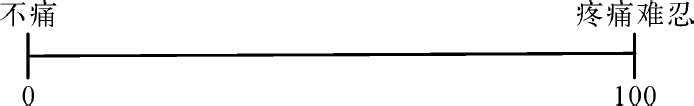
\includegraphics{./images/Image00227.jpg}
 \captionsetup{justification=centering}
 \caption{视觉模拟评分法}
 \label{fig21-1}
  \end{figure} 

(2)数字评分法(numeric rating
scale) 数字评分法是一个从0~10的点状标尺,0代表不疼,10代表疼痛难忍,由患者从上面选一个数字描述疼痛(图\ref{fig21-2})。其在评价老年患者急、慢性疼痛的有效性及可靠性上已获得证实。

\begin{figure}[!htbp]
 \centering
 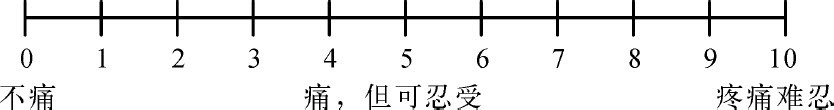
\includegraphics{./images/Image00228.jpg}
 \captionsetup{justification=centering}
 \caption{数字疼痛评分尺}
 \label{fig21-2}
  \end{figure} 

(3)面部表情评分法(faces pain
scale) 由6种面部表情及0~10分(或0~5分)构成,程度从不痛到疼痛难忍。由患者选择图像或数字来反映最接近其疼痛的程度(图\ref{fig21-3})。面部表情评分法与视觉模拟法、数字评分法有很好的相关性,可重复性也较好。

\begin{figure}[!htbp]
 \centering
 
\includegraphics{./images/Image00229.jpg}
 \captionsetup{justification=centering}
 \caption{面部表情疼痛评分法}
 \label{fig21-3}
  \end{figure} 

疼痛评估最可靠的方法是患者的主诉。视觉模拟法或数字评分法评分依赖于患者和医护人员之间的交流能力。当患者在较深镇静、麻醉或接受肌松剂情况下,常常不能主观表达疼痛的强度。在此情况下,患者的疼痛相关行为(运动、面部表情和姿势)与生理指标(心率、血压和呼吸频率)的变化也可反映疼痛的程度,可通过医护人员的观察进行疼痛评估,评估方法有疼痛行为量表(behavioral
pain scale)和重症监护疼痛观察工具法(critical care pain observation
tool),用于对不能自我报告疼痛患者的疼痛评估(表\ref{tab21-2},表\ref{tab21-3})。

\begin{table}[htbp]
{\centering
\caption{疼痛行为量表\textsuperscript{*}}
\label{tab21-2}
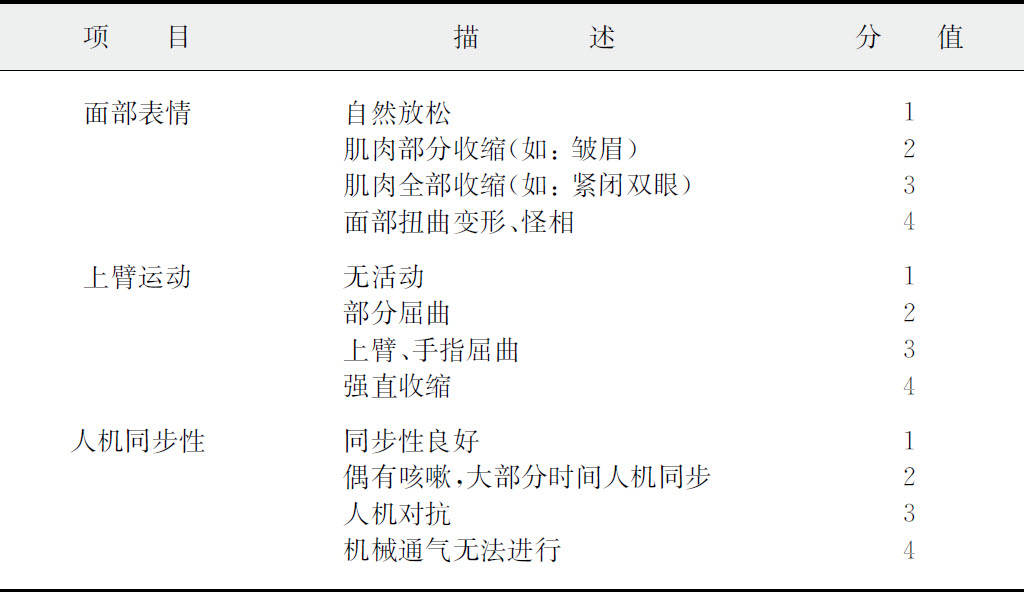
\includegraphics{./images/Image00230.jpg}}

\footnotesize * 目标3~4分。
\end{table}



\begin{table}[htbp]
{\begin{center}
\caption{重症监护疼痛观察工具法\textsuperscript{*}}
\label{tab21-3}
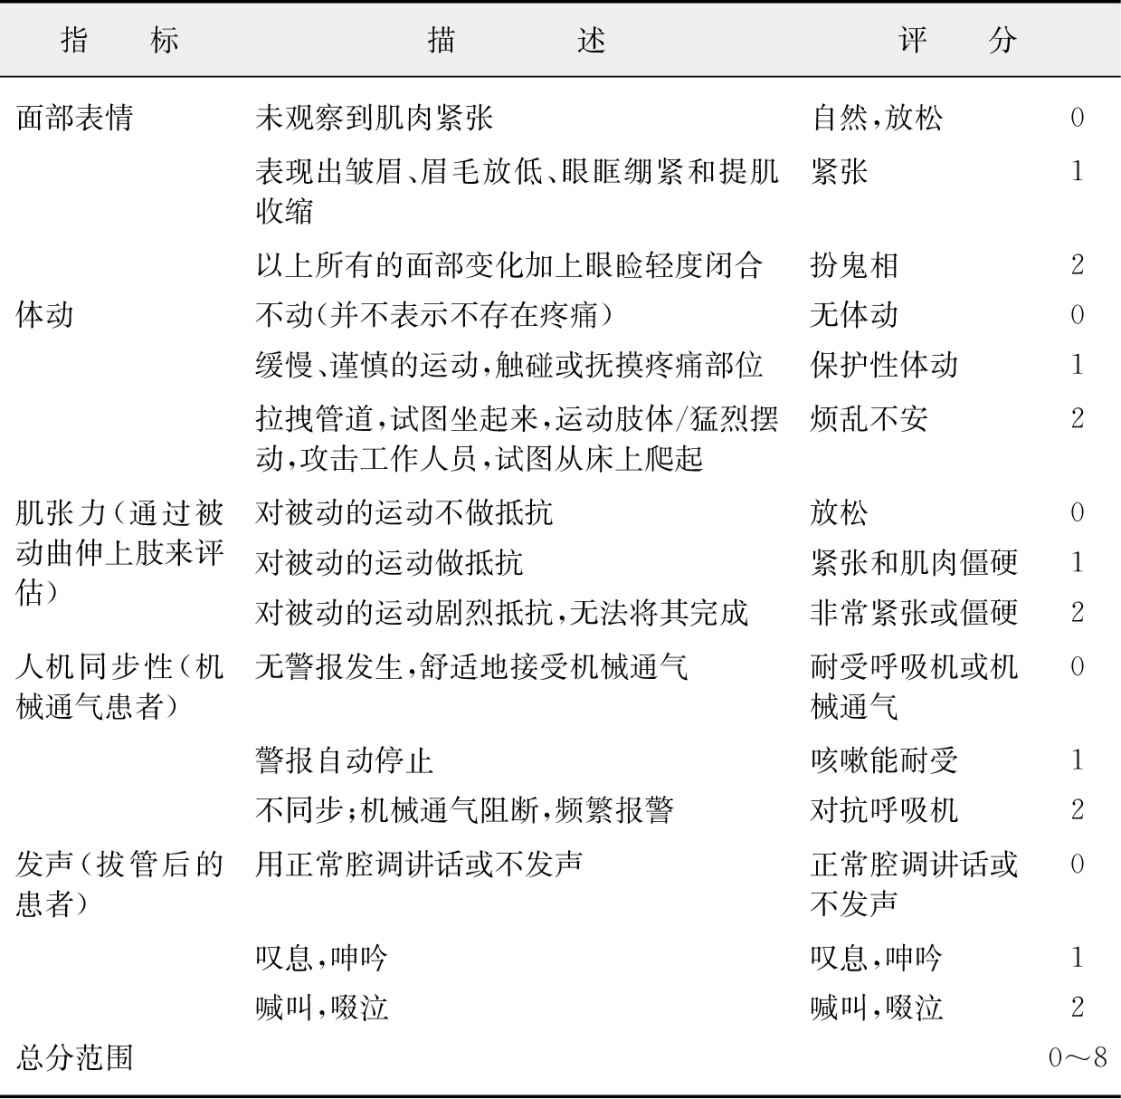
\includegraphics[width=\textwidth,height=\textheight,keepaspectratio]{./images/Image00231.jpg}
\end{center}
}

\footnotesize * 目标0~1分
\end{table}



\subsubsection{如何对重症患者进行镇静状态评估?}

定时评估镇静程度有利于调整镇静药物及其剂量以达到预期目标。理想的镇静评分系统应使各参数易于计算和记录,有助于镇静程度的准确判断并能指导治疗。目前临床常用的镇静评分系统有Ramsay评分、Riker镇静躁动评分,以及肌肉活动评分法等主观性镇静评分以及脑电双频指数等客观性镇静评估方法。

(1)镇静和躁动的主观评估

Ramsay评分:是临床上使用最为广泛的镇静评分标准,分为6级,分别反映3个层次的清醒状态和3个层次的睡眠状态(表\ref{tab21-4})。Ramsay评分被认为是可靠的镇静评分标准,但缺乏特征性的指标来区分不同的镇静水平。

\begin{table}[htbp]
\centering
\caption{Ramsay评分}
\label{tab21-4}
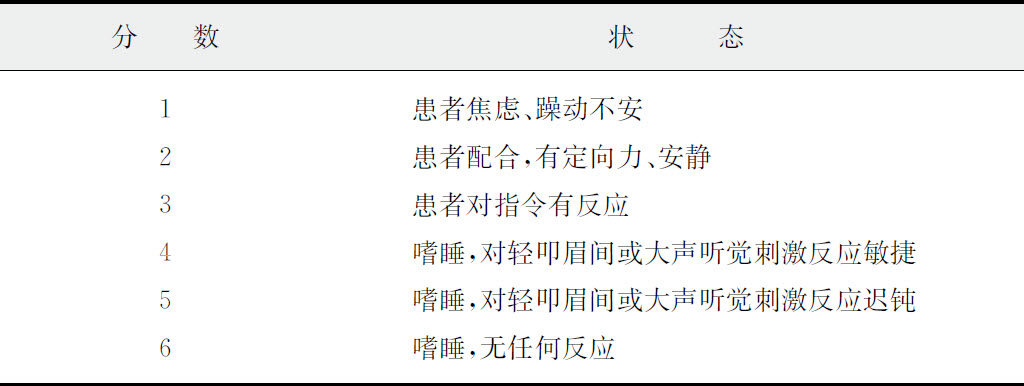
\includegraphics{./images/Image00232.jpg}
\end{table}

Riker镇静和躁动评分(sedation-agitation
scale):Riker镇静和躁动评分根据患者七项不同的行为对其意识和躁动程度进行评分(表\ref{tab21-5})。

\begin{table}[htbp]
\centering
\caption{Riker镇静和躁动评分}
\label{tab21-5}
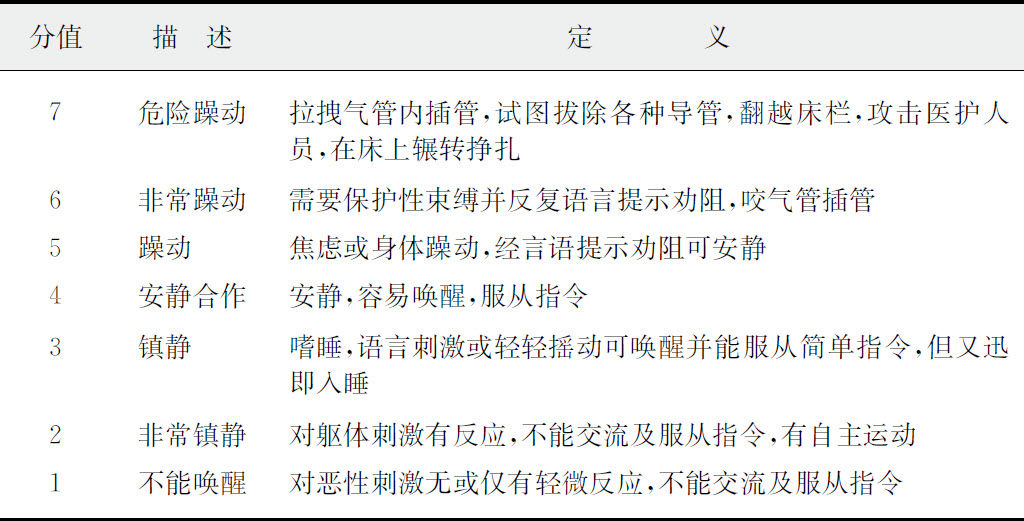
\includegraphics{./images/Image00233.jpg}
\end{table}

肌肉活动评分法(motor activity assessment
scale):自Riker镇静和躁动评分法演化而来,通过7项指标来描述患者对刺激的行为反应(表\ref{tab21-6})\footnote{* 恶性刺激是指吸痰或用力按压眼眶、胸骨或甲床5秒钟},对危重病患者也有很好的可靠性和安全性。

\begin{table}[htbp]
\centering
\caption{肌肉运动评分法}
\label{tab21-6}
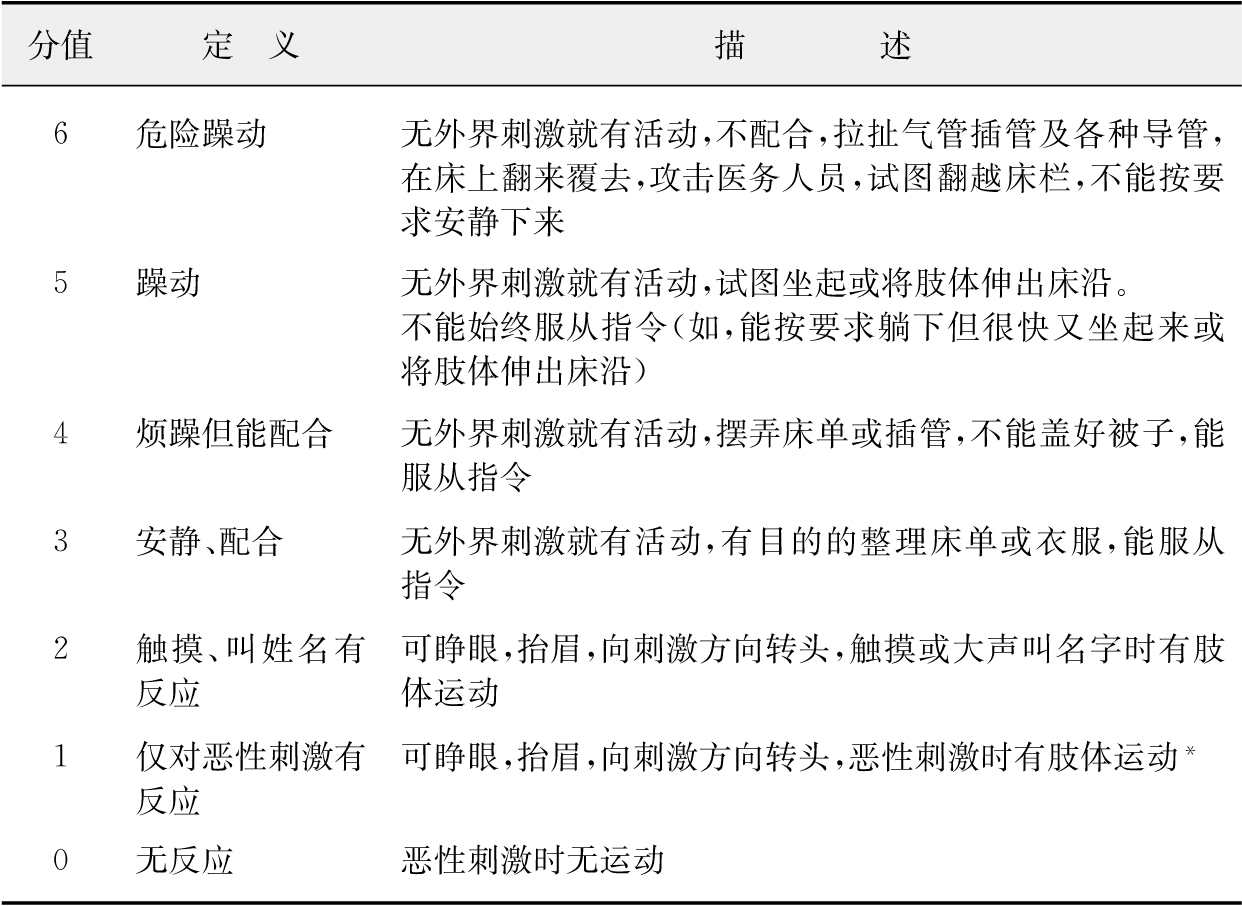
\includegraphics[width=\textwidth,height=\textheight,keepaspectratio]{./images/Image00234.jpg}
\end{table}



(2)镇静的客观评估 客观性评估是镇静评估的重要组成部分。但现有的客观性镇静评估方法的临床可靠性尚有待进一步验证。目前临床可用的方法主要是脑电双频指数(bispectral
index
scale)。脑电双频指数以0~100分表示从深度昏迷到完全清醒的不同程度,一般重症医学科中患者的镇静深度应维持于脑电双频指数值60~85分之间。

重症患者理想的镇静水平,是既能保证患者安静入睡又容易被唤醒。应在镇静治疗开始时就明确所需的镇静水平,定时、系统地进行评估和记录,并随时调整镇静用药以达到并维持所需镇静水平。

\subsection{常用镇静药物特点及应用}

\subsubsection{常用的镇静药物有哪些?}

理想的镇静药应具备起效快、剂量-效应可预测,半衰期短、无蓄积、停药后能迅速恢复,对呼吸循环抑制小,代谢方式不依赖肝肾功能及价格低廉等特点,但目前尚无药物能符合以上所有要求。重症医学科最常用的镇静药物为苯二氮䓬
类和丙泊酚(Propofol)。

(1)苯二氮䓬
类药物 重症医学科常用的苯二氮䓬
类药为咪唑安定(midazolam)、氯羟安定(lorazepam)及地西泮(diazepam)。

苯二氮䓬
类药物的作用存在较大的个体差异。老年患者、肝肾功能受损者药物清除减慢,肝酶抑制剂亦影响药物的代谢,故用药上需按个体化原则进行调整。苯二氮䓬
类药物负荷剂量可引起血压下降,尤其在血流动力学不稳定的患者;反复或长时间使用苯二氮䓬
类药物可致药物蓄积或诱导耐药的产生;该类药物有可能引起反常的精神作用。

苯二氮䓬
类药物有其相应的竞争性拮抗剂------氟马西尼(flumazenil),但应慎重使用,需注意两者的药效学和药动学差异,以免因拮抗后再度镇静而危及生命。

(2)丙泊酚 丙泊酚是一种广泛使用的静脉镇静药物,特点是起效快、作用时间短、撤药后可迅速清醒,且镇静深度呈剂量依赖性,镇静深度容易控制。丙泊酚亦可产生遗忘作用和抗惊厥作用。

丙泊酚单次注射时可出现暂时性呼吸抑制和血压下降、心动过缓,其对血压的影响与剂量相关,多见于心脏储备功能差、低血容量的患者。丙泊酚外周静脉注射可引起疼痛,故临床多采用持续缓慢静脉输注方式。另外,部分患者长期使用后可能出现诱导耐药。

丙泊酚的溶剂为乳化脂肪,提供热量4.6kJ/ml,长期或大量应用可能导致高甘油三酯血症;2%丙泊酚可降低高甘油三酯血症的发生率,因此更适宜于重症患者应用。老年人丙泊酚用量应减少。因乳化脂肪易被污染,故配制和输注时应注意无菌操作,单次药物输注时间不宜超过12小时。肝肾功能不全对丙泊酚的药代动力学参数影响不明显。

丙泊酚具有减少脑血流、降低颅内压、降低脑氧代谢率的作用。用于颅脑损伤患者的镇静可减轻颅内压的升高,而且丙泊酚半衰期短、停药后清醒快,有利于进行神经系统评估。此外,丙泊酚还有直接扩张支气管平滑肌的作用。

\subsubsection{咪唑安定有何特点?临床如何应用?}

咪唑安定(midazolam)又名速眠安,是当前临床应用的唯一水溶性苯二氮䓬
类镇静剂,同时具有脂溶性。该药能迅速穿透血脑屏障进入中枢神经系统,起效时间与安定相似(2.5分钟)。除静脉注射后快速再分布,使其作用维持短而便于持续静脉注射维持镇静外,其他方面与地西泮相似。长时间输注可使其作用时间延长。治疗开始时先给0.03mg/kg的负荷剂量,再以每小时0.03~0.13mg/kg的剂量维持,随时间延长逐渐调整速度。维持过程中,可追加负荷量以达到所需镇静水平。苯二氮䓬
类均可产生可靠的顺行性遗忘作用,无镇痛作用。

咪唑安定单剂静脉注射后,达到峰值血药浓度的时间为5~10分钟,作用持续时间30~120分钟,作用时间短的原因是由于快速分布到了外周组织,其清除半衰期约为4小时。活性代谢产物1羟基咪唑安定的药理活性为咪唑安定的60%~80%,肾功能正常患者的清除半衰期为1小时。咪唑安定持续静脉注射超过24小时时,停药后的镇静延续时间大大延长。若先2mg负荷量,继以5mg/小时维持3天,停药后作用至少持续24小时;若持续用药7天,停药后患者清醒时间将达2天甚至更长。

\subsubsection{地西泮的药理作用有哪些?主要用于哪些情况?}

地西泮,旧称安定(diazepam),是最早应用的静脉用镇静药,为长效脂溶性苯二氮䓬
类药物,能快速穿透血脑屏障进入中枢神经系统,主要作用于脑干网状结构和大脑边缘系统的苯二氮䓬
受体,产生抗焦虑、抗惊厥和肌松作用。静脉注射剂量为0.1~0.2mg/kg,2~3分钟内产生明显的镇静效应,3~5分钟达峰值效应;口服后吸收完全而迅速,30~60分钟血药浓度达峰值。地西泮单次静脉注射时因药物快速分布至外周组织而使作用很快减弱。地西泮的消除半衰期长达20~40小时,99%在肝脏中进行生物转化,其代谢产物具有与地西泮类似的药理学活性,而且半衰期更长,因此重复给药后可引起蓄积作用。肥胖者和老年人的分布容积增大,肝功能障碍时生物转化减慢,均可使地西泮的半衰期延长。

地西泮在危重病患者主要用于控制惊厥。由于以下原因,地西泮不再作为危重病患者镇静用常规药物:①地西泮的赋型剂中含丙二醇,刺激性较大,静脉和肌肉注射均可产生严重的注射痛,外周静脉注射易引起血栓性静脉炎;②除非每次给药前对患者的镇静水平进行客观评估,否则有计划地间断用药易引起镇静过度;③持续注射时需稀释,输入液体容量较大。

\subsubsection{何时考虑应用氯羟安定?}

氯羟安定,又名劳拉西泮(lorazepam),主要用于长时间镇静的危重病患者。氯羟安定为长效苯二氮䓬
类,较安定脂溶性差,因而外周蓄积的作用减低。与咪唑安定比较,氯羟安定作用持续时间长,低血压发生少,有相同的顺行性遗忘作用,此外,费用低、长时间用药后苏醒快也是其特点。氯羟安定因可间断静脉推注,亦可持续静脉输注,临床应用十分方便。氯羟安定的初始剂量为0.05mg/kg,根据需要每隔2~4小时给药一次。应注意的是,此药的用量个体差异非常大。因氯羟安定的起效时间慢,持续静脉输注时一般需单次或多次给予负荷量。

\subsubsection{常用的镇静药物应如何选择和应用?}

镇静药的给药方式应以持续静脉输注为主,首先应给予负荷剂量以尽快达到镇静目标。经肠道(口服、胃管、空肠造瘘管等)、肌肉注射则多用于辅助改善患者的睡眠。间断静脉注射一般用于负荷剂量的给予,以及短时间镇静且无需频繁用药的患者。

短期(<3天)镇静时,丙泊酚与咪唑安定产生的临床镇静效果相似。丙泊酚停药后清醒快,拔管时间明显早于咪唑安定,但未能缩短患者在重症医学科的停留时间。氯羟安定(劳拉西泮)起效慢,清除时间长,易发生过度镇静。因此,重症患者短期镇静宜主要选用丙泊酚与咪唑安定。

长期(>3天)镇静时,应首选氯羟安定。氯羟安定起效慢,作用持久,对循环、呼吸抑制作用较轻,长期应用的苏醒时间更有可预测性,且镇静满意率较高。因目前氯羟安定静脉制剂尚少,故亦可以丙泊酚和咪唑安定部分替代。丙泊酚与咪唑安定相比,丙泊酚苏醒更快、拔管更早,但丙泊酚较易出现低血压,而咪唑安定易发生呼吸抑制,用药期间咪唑安定可产生更多的遗忘。

为避免药物蓄积和药效延长,应在镇静过程中实施每日唤醒计划,即每日定时中断镇静药物输注(宜在白天进行),以评估患者的精神与神经功能状态,该方案可减少用药量,减少机械通气时间和重症医学科停留时间。但患者清醒期须严密监测和护理,以防止患者自行拔除气管插管或其他装置。

\subsection{睡眠障碍与焦虑}

\subsubsection{何谓睡眠障碍?如何保证重症患者的适当睡眠?}

睡眠是人体不可或缺的生理过程。睡眠障碍可能会延缓组织修复、减低细胞免疫功能。睡眠障碍的类型包括失眠、过度睡眠和睡眠觉醒节律障碍等。

失眠是一种睡眠质量或数量达不到正常需要的主观感觉体验,失眠或睡眠被打扰在重症医学科极为常见。原因包括:①持续噪音(来自仪器的报警,工作人员和设备);②灯光刺激;③高强度的医源性刺激(频繁的测量生命体征、查体,被迫更换体位);④疾病本身的损害以及患者对自身疾病的担心和不了解。患者在重症医学科睡眠的特点是短暂睡眠,醒觉和快速动眼睡眠交替。患者快动眼睡眠明显减少,非快动眼睡眠期占总睡眠时间的比例增加,睡眠质量下降,使得患者焦虑、抑郁或恐惧,甚至躁动,以致延缓疾病的恢复。

改善重症患者的睡眠首先应采用各种非药物措施,包括减少环境刺激、降低噪音,保证病房室内采光度,避免灯光直射患者,正常的昼夜节律,以及给予音乐和按摩治疗等。尽管如此,重症医学科内许多患者仍然可能存在睡眠困难,多数患者需要结合镇痛、镇静药物以改善睡眠。

\subsubsection{何谓谵妄?如何诊断?}

谵妄是多种原因引起的一过性的意识混乱状态。短时间内出现意识障碍和认知功能改变是谵妄的临床特征,意识清晰度下降或觉醒程度降低是诊断的关键。

重症患者因焦虑、麻醉、代谢异常、缺氧、循环不稳定、长时间置身于陌生而嘈杂的环境中等因素均可能导致谵妄,表现为精神状态突然改变或情绪波动,注意力不集中,思维紊乱和意识状态改变,伴或不伴有躁动状态。情绪低沉型谵妄往往预后较差,情绪活跃型谵妄比较容易识别,但也极易挣脱约束而出现意外
\protect\hyperlink{text00027.htmlux5cux23ch8-26}{\textsuperscript{{[}8{]}}}
。

谵妄的诊断主要依据临床检查及病史。目前推荐使用“重症医学科谵妄诊断的意识状态评估法(the
confusion assessment method for the diagnosis of delirium in the
ICU,CAM-ICU)”(表\ref{tab21-7})
\protect\hyperlink{text00027.htmlux5cux23ch6-26}{\textsuperscript{{[}6{]}}}
。

\begin{table}[htbp]
{\begin{center}
\caption{重症医学科谵妄诊断的意识状态评估法\textsuperscript{*}}
\label{tab21-7}
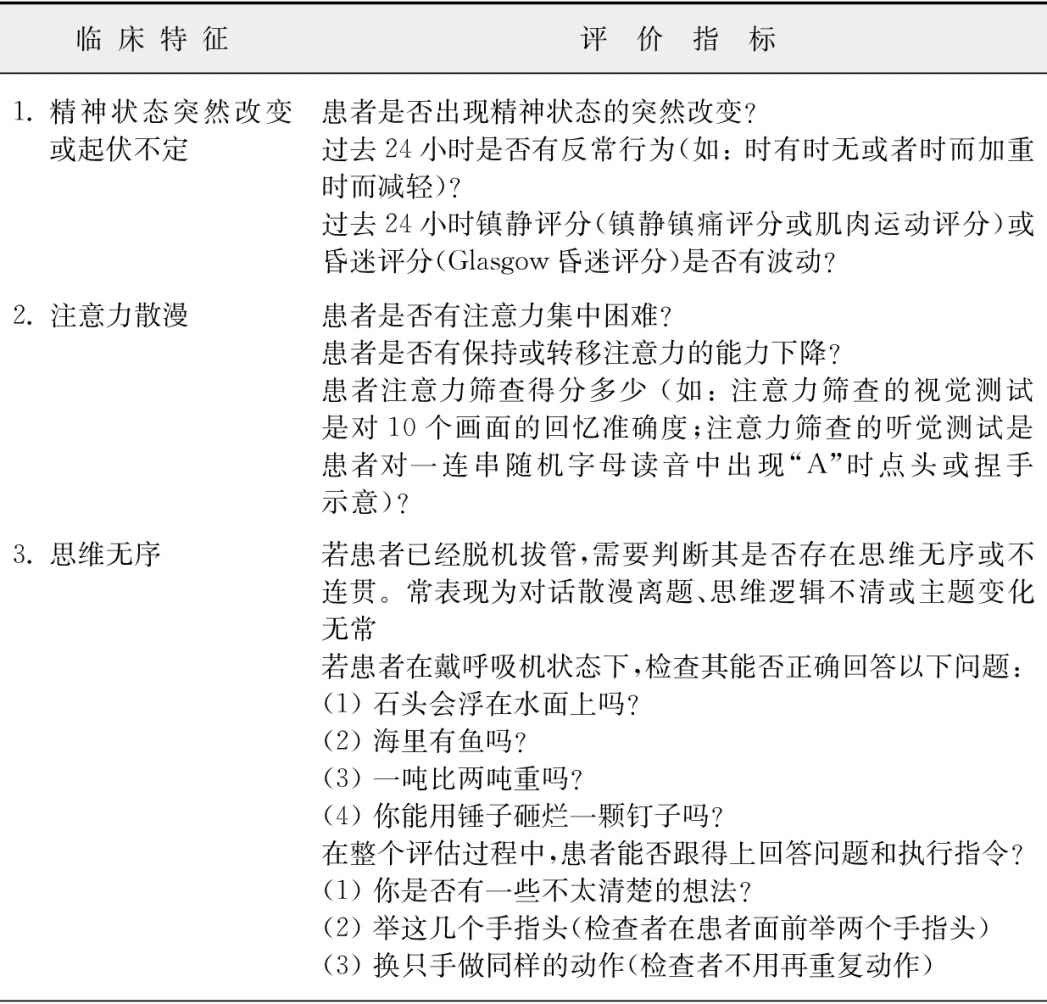
\includegraphics[width=.9\textwidth,height=\textheight,keepaspectratio]{./images/Image00247.jpg}
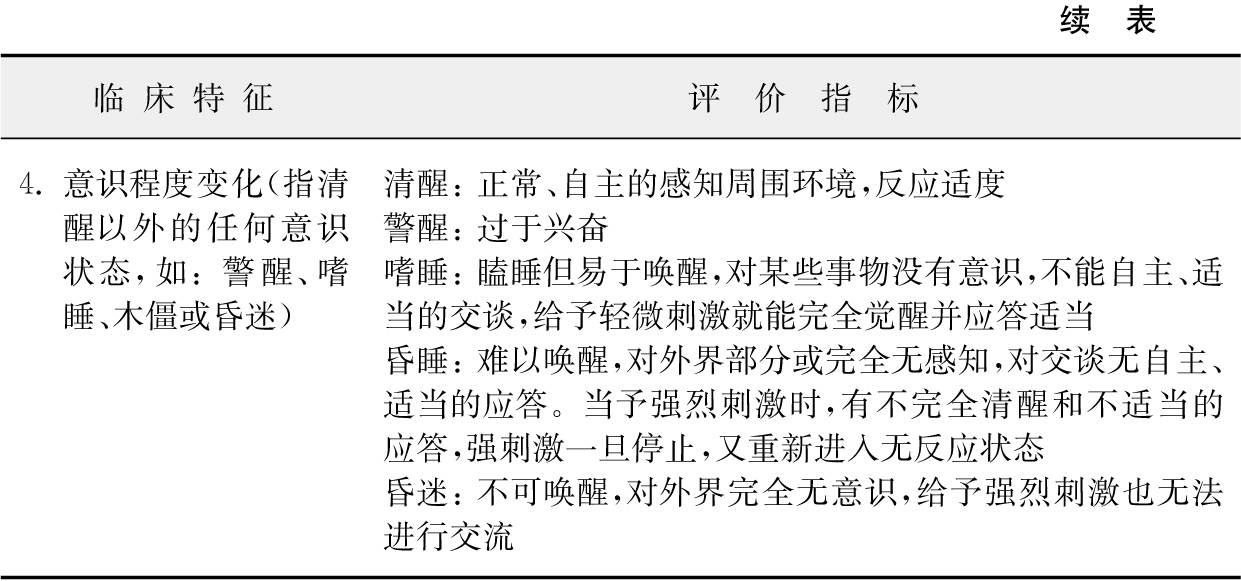
\includegraphics[width=.9\textwidth,height=\textheight,keepaspectratio]{./images/Image00248.jpg}
\end{center}
}

\footnotesize * 若患者有特征1和2,或者特征3,或者特征4,就可诊断为谵妄。
\end{table}





\subsubsection{谵妄治疗的首选药物是什么?治疗中应该注意哪些问题?}

谵妄状态必须及时治疗。一般应少用镇静药物,以免加重意识障碍。但对于躁动或有其他精神症状的患者则必须立即给药予以控制,防止意外发生。当然,镇痛镇静药使用不当可能会加重谵妄症状。

氟哌啶醇(haloperidol)为重症医学科成年重症患者谵妄治疗的首选药物。由于阿片类或苯二氮䓬
类可进一步加重患者感觉障碍而发生锥体外系症状,所以不作为谵妄时首选药物。

氟哌啶醇属丁酰苯类神经安定药,静脉注射安全,可达最大生物利用度。通常初始剂量为2~10mg,间隔2~4小时可重复给药。静脉注射后30~60分钟达临床效果,持续4~8小时。

对于谵妄和躁动的患者间断用药的缺点是注射后达峰值血药浓度时,可能产生相对的过度镇静,而药效逐渐减退时因再发躁动,患者出现发作性心率加快、血压升高及氧耗增加。这种躁动和过度镇静的周期性交替不利于呼吸机的脱机和患者主动参与治疗。因此,持续静脉注射可能是一种值得推广的方法。

持续注射氟哌啶醇的指征为24小时内需单剂注射10mg氟哌啶醇超过8次,或连续5小时的剂量超过10mg/小时。具体用法为:首剂10mg,然后以10mg/小时维持,如症状未控制,每隔30分钟可重复注射10mg,同时每次增加注射速度5mg/小时,并可考虑加用苯二氮䓬
类药物。一旦谵妄或焦虑控制且24小时中很少甚至不需单剂注射,则减量一半。Ramsay评分≥6分时,应停药。需要时再单剂注射。

氟哌啶醇可致心电图QT间期延长,与其他延长QT间期的药物合用时应注意。少数患者可有锥体外系症状。

\subsection{镇痛与肌松}

\subsubsection{常用镇痛药物有哪些?临床怎么选择?}

理想的镇痛药物应具有起效快、易调控、用量少、较少的代谢产物蓄积及费用低廉的优点。临床所用的镇痛药物主要包括阿片类镇痛药和非甾体抗炎药。

(1)阿片类镇痛药 ①重症患者的持续镇痛宜首选吗啡。②芬太尼不宜用于维持镇痛,虽然其镇痛效价是吗啡的100~180倍,静脉注射后起效快、作用时间短、对循环的抑制较吗啡轻,但其清除半衰期较吗啡显著延长,重复用药后可导致明显的蓄积和延时效应。快速静脉注射芬太尼可引起胸壁、腹壁肌肉僵硬而影响通气。③瑞芬太尼是新的短效μ受体激动剂,在重症医学科可用于患者短时间的镇痛,多采用持续输注。瑞芬太尼代谢途径是被组织和血浆中非特异性酯酶迅速水解。代谢产物经肾排出,清除率不依赖于肝肾功能。在部分肾功不全患者的持续输注中,不会发生蓄积作用。该药对呼吸有抑制作用,但停药后3~5分钟恢复自主呼吸。④舒芬太尼的镇痛作用为芬太尼的5~10倍,作用持续时间为芬太尼的两倍。一项与瑞芬太尼的比较研究证实,舒芬太尼在持续输注过程中随时间延长,剂量减少,但唤醒时间延长。

阿片类药物的副作用主要是引起呼吸抑制、血压下降和胃肠蠕动减弱,在老年人尤其明显。阿片类药诱导的意识抑制可干扰对重症患者的病情观察,在一些患者还可引起幻觉、加重烦躁。

重症患者不推荐使用哌替啶镇痛。哌替啶(度冷丁)镇痛效价约为吗啡的1/10,大剂量使用时,可导致神经兴奋症状(如欣快、谵妄、震颤、抽搐),肾功能障碍者发生率高,可能与其代谢产物去甲哌替啶大量蓄积有关。哌替啶禁忌和单胺氧化酶抑制剂合用,否则两药联合使用可出现严重副反应。

(2)非甾体类抗炎镇痛药(NSAIDs) 这类药物的作用机制是通过非选择性、竞争性抑制前列腺素合成过程中的关键酶------环氧化酶而达到镇痛效果。代表药物主要为对乙酰氨基酚。

该类药物可用于治疗轻度至中度疼痛,和阿片类联合使用时有协同作用,可减少阿片类药物的用量,并可用于缓解患者长期卧床的轻度疼痛和不适。对乙酰氨基酚对肝衰竭或营养不良造成的谷胱甘肽储备枯竭的患者易产生肝毒性,应予警惕。对于那些有明显饮酒史或营养不良的患者使用对乙酰氨基酚剂量应<2g/天,其他情况<4g/天。

\subsubsection{吗啡有什么特点?怎么使用?}

吗啡(morphine)是重症患者首选的镇痛剂,具有价廉、强效、欣快感的优点。正常人静脉注射后半衰期为1.5~2小时,在重症医学科的危重病患者吗啡的分布容积和蛋白结合力可能发生变化,导致其作用效应放大,作用时间延长。但吗啡有组织胺释放作用,在有效循环血量不足或心血管功能明显抑制的患者,大剂量应用时可能引起低血压。

吗啡应静脉注射给药,可采用持续注射或间断注射两种方法,根据镇痛效应和镇痛目标调整用药剂量。持续注射给药时,先给予0.03~0.2mg/kg负荷剂量,再以1~3mg/小时维持,通常需按负荷剂量间断追加给药。短时间镇痛时,可选用间断注射的方法用药,根据镇痛要求每间隔1~2小时重复给药。

\subsubsection{芬太尼的药理作用是什么?有何特点?}

对于血流动力学不稳定的重症患者应当首选芬太尼(fentanyl)。芬太尼无组胺释放作用,因而用于血流动力学不稳定患者更为安全。芬太尼为合成类阿片制剂,临床镇痛强度为吗啡的75~125倍。该药脂溶性很高,易于透过血脑屏障而进入脑组织,也易于从脑重新分布至外周组织,尤其是肌肉和脂肪组织,因此起效更快,单剂静脉注射时半衰期仅30~60分钟,作用时效短暂。但在长时间持续应用的患者,外周组织的蓄积可使半衰期增至9~16小时,撤药时应逐步减量。芬太尼无催眠作用,代谢产物无活性,与吗啡无交叉过敏现象。

由于其药代动力学特点,芬太尼反复注射或大剂量注射后,可在用药后3~4小时出现迟发性呼吸抑制。快速静脉注射可引起胸壁和腹壁肌肉僵硬而影响通气。在没有机械通气支持的患者,应予高度重视。

芬太尼一般持续静脉注射,开始治疗时先静脉推注1~3μg/kg的负荷剂量,继以每小时1~3μg/kg维持,必要时可间断追加1μg/kg的负荷剂量。床边行短时操作如换药、气管切开时,间断静脉推注1~3μg/kg的芬太尼,可产生满意的镇痛效果。

\subsubsection{瑞芬太尼与芬太尼有何不同之处?}

瑞芬太尼为芬太尼类μ型阿片受体激动剂,在人体内1分钟左右迅速达到血脑平衡,在组织和血液中被迅速水解,故起效快,维持时间短,与其他芬太尼类似物明显不同。瑞芬太尼的镇痛作用及其副作用呈剂量依赖性,与催眠药、吸入性麻醉药和苯二氮䓬
类药物合用有协同作用。瑞芬太尼的μ型阿片受体激动作用可被纳洛酮所拮抗。瑞芬太尼也可引起呼吸抑制、骨骼肌(如胸壁肌)强直、恶心、呕吐、低血压和心动过缓等,在一定剂量范围内,随剂量增加而作用加强。盐酸瑞芬太尼剂量高达30μg/kg静脉注射(1分钟内注射完毕)不会引起血浆组胺浓度的升高。瑞芬太尼代谢不受血浆胆碱酯酶及抗胆碱酯酶药物的影响,不受肝、肾功能及年龄、体重、性别的影响,主要通过血浆和组织中非特异性酯酶水解代谢,大约95%的瑞芬太尼代谢后经尿排泄,主代谢物活性仅为瑞芬太尼的1/4600。本品长时间输注给药或反复注射用药其代谢速度无变化,体内无蓄积。

\subsubsection{哌替啶的作用机制是什么?}

哌替啶(pethidine)的商品名为度冷丁,镇痛强度仅为吗啡的1/10,作用持续时间为吗啡的1/2~3/4。大剂量度冷丁常可引起中枢神经系统兴奋,表现为谵妄、瞳孔散大、抽搐等,主要与其代谢产物苯哌利啶在体内蓄积有关,在合并有肾衰竭的患者尤易发生。度冷丁的成瘾性较其他阿片类镇痛药强。小剂量的度冷丁能有效控制寒战。因此,度冷丁不作为危重病患者的常规镇痛用药,但用于外科术后疼痛伴寒战的患者,具有独特的效果。

\subsubsection{为什么吗啡应作为重症患者持续镇痛的一线药物?}

作为镇痛治疗的药物应该具有既能快速起效缓解疼痛,又能尽量减少体内组织蓄积、及时从体内排除的特点,即所谓“进得去,出得来”。

临床常用的几种阿片类镇痛药物主要包括度冷丁、芬太尼及吗啡。度冷丁(哌替啶)因其代谢产物甲基度冷丁的半衰期长逾30多小时,且对肝脏有损害作用,已日益减少其在临床的应用。芬太尼虽然有较短的分布半衰期,但其清除半衰期却是吗啡的2倍以上,因此在维持患者镇痛、反复给药时,其组织蓄积增加,会导致镇痛镇静时间延长,患者苏醒和脱离呼吸机延迟等不利结果。吗啡的分布半衰期虽长于芬太尼,但其清除半衰期较短,适合用于需较长时间维持镇痛治疗的患者。因此,目前国际上对于重症患者的维持镇痛治疗,已基本弃用度冷丁,对于血流动力学不稳定或肾功能障碍患者可考虑应用芬太尼,而将吗啡作为大部分情况下维持镇痛治疗的一线药物。

瑞芬太尼是近年来推出的新的阿片类镇痛药物,其所具有的起效快、组织蓄积少、剂量-效应曲线明确等特点已开始引起人们的关注,但由于价格较昂贵,目前在临床上尚未得到大规模应用,还有待进一步评价。

\subsubsection{镇痛与镇静治疗的关系如何?有兼镇痛、镇静双重作用的药物吗?}

镇痛是镇静治疗的基础,疼痛因素得不到祛除,镇静治疗就不可能有效;反之,仅有镇痛而未配合镇静,其他焦虑恐惧的因素未得到有效祛除,也不能达到减轻应激反应的目的。因此,镇痛镇静治疗往往需联合进行,不能相互替代。

阿片类镇痛药物和大多数镇静药物联合应用时,均具有相加或协同作用,可以降低各自的药物剂量,从而减少各自药物的副作用。

近年来,一种兼有镇痛与镇静双重功效的新型α\textsubscript{2}
受体激动剂右美托咪定(dexmedetomidine)正日益引起人们的重视。

α\textsubscript{2}
受体激动剂有很强的镇静、抗焦虑作用,且同时具有镇痛作用,可减少阿片类药物的用量,其亦具有抗交感神经作用,可导致心动过缓和(或)低血压。

右美托咪定(dexmedetomidine)由于其α\textsubscript{2}
受体的高选择性,是目前唯一兼具良好镇痛与镇静作用的药物,同时它没有明显心血管抑制及停药后反跳,其半衰期较短,可单独应用,也可与阿片类或苯二氮䓬
类药物合用。有研究显示,右美托咪啶能达到良好的镇静效果,同时降低机械通气时间,并减少谵妄的发生。

\subsubsection{右美托咪定药理作用是什么?有何特点?}

右美托咪定是美托咪啶的右旋异构体,属咪唑类衍生物,其作用时间很短,静脉注射快速分布半衰期大约6分钟,消除半衰期为2.0~2.5小时,并且具有高蛋白结合率(94%)和较大的分布容积(1.33L/kg),大部分由肝脏代谢,肝功能损伤患者其消除率下降,且变异度较大,所以肝功能损伤患者应适当减少用量。肾衰竭患者对该药的血浆蛋白结合率和药代学参数无明显变化,无需调整剂量。

右美托咪定是一种高选择性的α\textsubscript{2}
受体激动剂,其与α\textsubscript{2} 和α\textsubscript{1}
受体的亲和力比率为1620∶1,通过作用于蓝斑核和脊髓的α\textsubscript{2}
肾上腺素受体,发挥镇静、抗焦虑作用,同时也具有镇痛作用。在联合用药时可以减少阿片类药物的用量,并且无呼吸抑制。右美托咪定通过抗交感作用减少去甲肾上腺素的释放,减少患者心动过速和高血压的发生,减少患者对气管插管的应激反应,维持患者血流动力学的稳定。

\subsubsection{为什么应尽量避免肌松药物的使用?}

在镇痛镇静不足时,应用肌松药物可以掩盖患者的镇静状态,这种“清醒肌松”反而会造成患者的极度恐惧与紧张,交感神经的极度兴奋,患者可表现为血压高、心率快,此时不要盲目给予药物降低血压或减慢心率,应结合临床综合评估,给予充分镇痛和镇静治疗后观察变化,并酌情采取进一步的治疗措施。切忌未予镇痛、镇静基础治疗即直接应用肌松药物。

一般而言,绝大多数的重症患者依靠镇痛与镇静治疗即可达到有效的镇静,极少需要应用肌松药物。除破伤风等强烈而持续的惊厥发作、肌肉强直抽搐,以及个别极端的呼吸模式(如反比通气)和极其严重的“人机对抗”情形之外,应尽量避免应用肌松剂。

长时间制动、长时间神经肌肉阻滞治疗使患者关节和肌肉活动减少,瞬目不能,并增加压疮和深静脉血栓形成的危险,为此应给予积极的物理治疗预防深静脉血栓形成,并保护眼睛以及关节和肌肉的运动功能。

\subsection{长期镇静}

\subsubsection{为什么对长期镇静患者需要实行每日唤醒策略?}

长期镇静的患者,为了观察其神志、感觉、运动和反射,需要每日临时停止镇静药物的给予,予以唤醒。同时,每日唤醒的时段还可以令患者主动呛咳和肢体运动,利于有效地清除气道坠积的分泌物,防止深静脉血栓的形成和压疮的发生。

一般可在每日清晨暂时停止镇静药物泵注,使得晨间交班时可以唤醒患者,观察其神志及感觉运动变化,帮助其咯痰和活动肢体;然后再给以负荷量的一半静脉推注后继续持续泵注以维持镇静。国外随机对照的临床研究表明,实施每日唤醒的患者与对照组患者相比,其机械通气时间、重症医学科留治时间、苯二氮䓬
类镇静药物和镇痛药物用量,以及住院总费用都有明显的下降
\protect\hyperlink{text00027.htmlux5cux23ch7-26}{\textsuperscript{{[}7{]}}}
。

\subsubsection{镇静药物长期使用时应注意哪些问题?}

长期使用镇痛镇静药物的患者,应注意药物的耐受及其与其他药物的相互作用;在撤离治疗时应强调平稳安全,避免在撤离过程中出现戒断症状和(或)反跳现象。

丙泊酚与咪唑安定长期使用(超过1~2周)时均有可能出现耐受,此时一方面可以逐渐酌情增加剂量,或配伍联合用药,以保证镇静效果;另一方面则应积极再次评估患者的病情,尽可能祛除所有导致焦虑躁动的诱因,大部分患者此时已有可能停止镇静治疗。

在停止镇静时,丙泊酚由于其良好的量效反应曲线,往往较快苏醒,而咪唑安定等苯二氮䓬
类药物由于其脂溶性组织蓄积的特点,在停药时有可能出现躁动,此时可考虑临时追加咪唑安定,或临时辅以小量丙泊酚,待蓄积的苯二氮䓬
类药物清除后停药,使患者安全苏醒。

长期应用丙泊酚镇静时必须经常监测血清甘油三酯水平,以免血脂廓清障碍导致高甘油三酯血症。重症患者长期镇静需用丙泊酚时,应首选浓度为2%的丙泊酚制剂,以减少脂肪乳剂的输注量。

\begin{center}\rule{0.5\linewidth}{\linethickness}\end{center}

参考文献

\protect\hyperlink{text00027.htmlux5cux23ch1-26-back}{{[}1{]}} .Novaes
MA,Knobel E,Bork AM,et al.Stressors in ICU:Perception of the
patient,relatives and health care team.Intensive Care
Med,1999,25:1421-1426.

\protect\hyperlink{text00027.htmlux5cux23ch2-26-back}{{[}2{]}} .Jacobi
J,Fraser GL,Coursin DB,et al.Clinical practice guideline for the
sustained use of sedatives and analgesics in the critically ill
adult.Crit Care Med,2002,30:119-141.

\protect\hyperlink{text00027.htmlux5cux23ch3-26-back}{{[}3{]}}
.中华医学会重症医学分会:中国重症加强治疗病房患者镇痛和镇静指导意见.中华外科杂志,2006,44:1158-1166.

\protect\hyperlink{text00027.htmlux5cux23ch4-26-back}{{[}4{]}} .Epstein
J,Breslow MJ.The stress response of critical illness.Crit Care
Clin,1999,15:17-33.

\protect\hyperlink{text00027.htmlux5cux23ch5-26-back}{{[}5{]}} .Caroll
KC,Atkins PJ,Herold GR,et al.Pain assessment and management in
critical ill postoperative and trauma patients:A multisite study.Am J
Crit Care,1999,8:105-117.

\protect\hyperlink{text00027.htmlux5cux23ch6-26-back}{{[}6{]}} .Lewis
KS,Whipple JK,Michael KA,et al.Effect of analgesic treatment on the
physiological consequences of acute pain.Am J Hosp
Pharm,1994,51:1539-1554.

\protect\hyperlink{text00027.htmlux5cux23ch7-26-back}{{[}7{]}} .Ely
EW,Margolin R,Francis J,et al.Evaluation of delirium in critically
ill patients:Validation of the confusion assessment method for the
intensive care unit(CAMICU).Crit Care Med,2001;29:1370-1379.

\protect\hyperlink{text00027.htmlux5cux23ch8-26-back}{{[}8{]}} .Kress
J,Pohlman A,O'Connor M,et al.Daily interruption of sedative
infusions in critically ill patients undergoing mechanical
ventilation.N Engl J Med,2000,342:1471-1477.

\protect\hypertarget{text00028.html}{}{}

